\documentclass[12pt]{amsart}

\usepackage[margin=3.5 cm]{geometry}
\usepackage{graphicx, mathabx}
\usepackage{color}
\usepackage{graphicx}
\usepackage{float}
\graphicspath{ {./images/} }
\linespread{1.5}
\newcommand{\vect}[1]{\mathbf{#1}}
\begin{document}
\title[STAT339 - Machine Learning]{STAT 339 - Homework 1b (Linear Regressions)}

\author{Peng Gu, Liam Axon, Xiaoyun Gong} 
\date{\today}

\maketitle

\section*{Exercise 1}

\subsection*{part(b)}

We applied our own OLS solver to the ``womens100.csv'' data set, with the results shown below:

\begin{figure}[H]
    \centering
    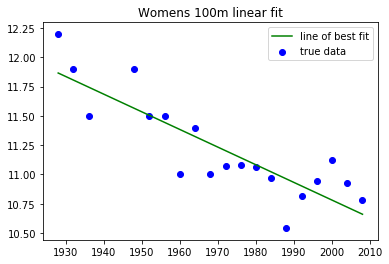
\includegraphics[scale=0.8]{Figure_womesn100.png}
    \caption{Graph of ``womens100.csv'' best fit}
    \label{fig:my_label}
\end{figure}

The line shown on the graph is $y = w_0 + w_1 x$ where $w_0 = 40.09$ and $w_1 = -0.015$.

We compared this to the line given in the textbook, which has $w_0 = 40.92$ and $w_1 = -0.015$.

These values are very close, and tell us that our regression solver is correctly finding a line of best fit.

\subsection*{part(c)}

Our algorithm predicted a value for the 2012 Olympics of 10.647, and it predicted a value for the 2016 Olympics of 10.593s. The actual racetime for 2012 is 10.75s, and the actual racetime for 2016 is 10.71s. These are both a little high of the actual value, but the difference is not prominent.

In fact, the squared prediction error for 2012 is 0.0106 and the squared prediction error for 2016 is 0.0136.

\subsection*{part(g)}

When we applied our polynomial regression solver to the ``synthdata2016.csv'' data set, looking for a cubic of best fit, we got the following:

\begin{figure}[H]
    \centering
    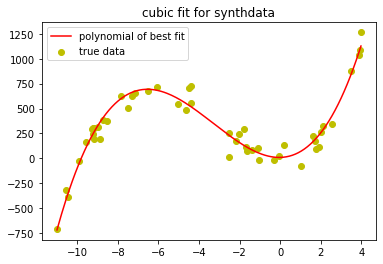
\includegraphics{Figure_synthdata.png}
    \caption{Graph of ``synthdata2016.csv'' best fit}
    \label{fig:my_label}
\end{figure}

\newpage

\section*{Exercise 3}
\subsection*{part(a)}
\begin{proof}
Let $f,g:\mathbb{R}^N\to\mathbb{R}^M$,  $\vect{v}\in\mathbb{R}^N$, and $a = f(\vect{v})^T g(\vect{v})\in \mathbb{R}$.
\begin{align*}
    \frac{da}{d\vect{v}} &= \frac{d}{d\vect{v}}(f(\vect{v})^T g(\vect{v}))\\
    &= \frac{d}{d\vect{v}} \sum_{i=1}^M (f_i(\vect{v})g_i(\vect{v}))\\
    &= \sum_{i=1}^M \frac{d}{d\vect{v}}(f_i(\vect{v})g_i(\vect{v}))\\
    &= \sum_{i=1}^M (f_i(\vect{v})\frac{dg_i}{d\vect{v}}+g_i(\vect{v})\frac{df_i}{d\vect{v}})\\
    &= \sum_{i=1}^M f_i(\vect{v})\frac{dg_i}{d\vect{v}} +\sum_{i=1}^M g_i(\vect{v})\frac{df_i}{d\vect{v}}\\
    &= f(\vect{v})^T\frac{dg}{d\vect{v}} +g(\vect{v})^T\frac{df}{d\vect{v}}
\end{align*}
\end{proof}

\subsection*{part(b)}
\begin{proof}
Let $g:\mathbb{R}^N\to\mathbb{R}^N$, $g(\vect{v})=\vect{A}\vect{v}$, and let $f=\textbf{I}$.
\begin{align*}
    \frac{d}{d\vect{v}}\vect{v}^T\vect{A}\vect{v}
    = \frac{d}{d\vect{v}}f(\vect{v})^T g(\vect{v})
    &=f(\vect{v})^T \frac{dg}{d\vect{v}}
    + g(\vect{v})^T  \frac{df}{d\vect{v}}\\
    &= f(\vect{v})^T \vect{A}
    +g(\vect{v})^T\vect{I}\\
&= \vect{v}^T\vect{A}+(\vect{A}\vect{v})^T\\
&= \vect{v}^T\vect{A} + \vect{v}^T\vect{A}^T\\
&= \vect{v}^T\vect{A} + \vect{v}^T\vect{A}\\
&= 2\vect{v}^T\vect{A}
\end{align*}
\end{proof}
\section*{Exercise 4}
We need to find the derivative first:
\begin{align*}
   \frac{d\mathcal{L}}{d\vect{w}}&=\frac{1}{N}[
   (\vect{t}-\vect{Xw})^T \frac{d}{d\vect{w}}(\vect{A(t-Xw)}) +
   (\vect{A(t-Xw)})^T \frac{d}{d\vect{w}}(\vect{t}-\vect{Xw})
   ]\\
   &= \frac{1}{N}[(\vect{t}-\vect{Xw})^T(-\vect{AX})+ \vect{(t-Xw)}^T\vect{A}^T(-\vect{X})]\\
   &\mbox{(Note that $\vect{A}$ is symmetric, so $\vect{A}^T = \vect{A}$.)}\\
   & = -\frac{1}{N}[\vect{(t-Xw)}^T\vect{AX}+\vect{(t-Xw)}^T\vect{AX}]\\
   & = -\frac{2}{N}[\vect{(t-Xw)}^T\vect{AX}]
\end{align*}
Now, set $ \frac{d\mathcal{L}}{d\vect{w}}$ to $0$:
\begin{align*}
    -\frac{2}{N}[\vect{(t-Xw)}^T\vect{AX}]&=0\\
    \vect{(t-Xw)}^T\vect{AX}&=0\\
    (\vect{t}^T-\vect{w}^T\vect{X}^T)\vect{AX}&=0\\
    \vect{t}^T\vect{AX}-\vect{w}^T\vect{X}^T\vect{AX}&=0\\
    \vect{w}^T\vect{X}^T\vect{AX} &=\vect{t}^T\vect{AX}\\
    \vect{w}^T&=\vect{t}^T\vect{AX}(\vect{X}^T\vect{AX})^{-1}\\
    \vect{w} &= ((\vect{X}^T\vect{AX})^{-1})^{T}\vect{X}^T\vect{A}^T\vect{t}\\
    \vect{w} &= ((\vect{X}^T\vect{AX})^{T})^{-1}\vect{X}^T\vect{A}^T\vect{t}\\
    \mbox{(Again, note that $\vect{A}$}&\mbox{  is symmetric, so $\vect{A}^T = \vect{A}$.)}\\
    \vect{w} &=(\vect{X}^T\vect{AX})^{-1}\vect{X}^T\vect{A}\vect{t}
\end{align*}
\end{document}

